\chapter{Surface Event Pulse Shape Simulations}

%\section{Surface Alphas}

% \subsection{Properties of Alpha Interactions}
% Alpha particles are composed of two protons and two neutrons tightly bound together. They are identical to ionized Helium ions and carry a charge of $+2$ e. The energy of alpha particles is correlated with the half-life of the parent isotope, such that the ones with the highest energies are from parent atoms with the shortest half-lives. Thus, the energies of alpha particles are normally between about $4$ and $6$ MeV. For a given material, the linear stopping power S is defined as $-\frac{dE}{dx}$. The energy loss of charged particles in a material is then given by the Bethe formula:

% \begin{equation}\label{bethe_formula}
%     -\frac{dE}{dx} = \frac{4\pi e^4z^2}{m_0\nu^2}NB
% \end{equation}

% such that

% \begin{equation}\label{bethe_B}
%     \text{B}=Z\left[ \text{ln}\frac{2m_0\nu^2}{I}-\text{ln}\right(1-\frac{\nu^2}{c^2}\left)-\frac{\nu^2}{c^2}\right]
% \end{equation}

% Here $\nu$ and $ze$ are the charges of the given particle, N and Z are
% the number density and the atomic number of the absorber atoms, and  m$_0$ and e are the rest mass and charge of electron respectively. Parameter I represents the average excitation and ionization potential of the absorber and is normally determined experimentally. Eq. \ref{bethe_formula} suggests that the energy loss for non-relativistic particles is proportional to $1/\nu^2$, or the kinetic energy. This can be understood by noting that the smaller the velocity, the longer the particles spend in the vicinity of electrons of the material's atoms, and the higher the energy loss. Eq. \ref{bethe_formula} is proportional to z$^2$ for constant velocity. Thus heaver particles will have more energy loss for a given velocity. This results in alphas having a very low penetration depth, usually around $10$ micrometers.

% Energy loss of alpha particles can be best understood by plotting specific energy loss along the track. The plot known as the Bragg curve is shown in Fig. \ref{bragg_curve_fig}. During most of the track, the energy loss increases roughly as 1/E as predicted by Eq.\ref{bethe_formula}. As the particles slow down, electron pickup reduces the charge and the curve falls off. A result of these curves is that alpha deposits a large amount of energy in a very localized area. For Germanium, the penetration depth of alpha particles is about $17.6$ - $20.0$ microns. The n+ electrode and p+ electrode in LEGEND detectors are too thick for alphas to penetrate and deposit much energy. However, the passivated surface experiences complex surface effects which are described next.

% \begin{figure}
% \centering
% 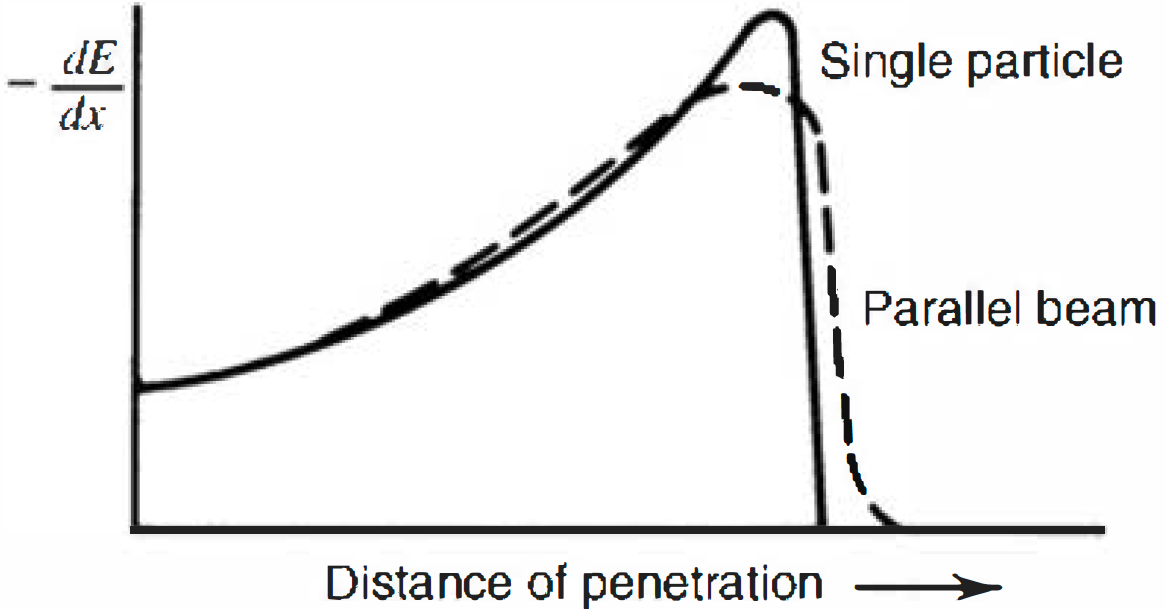
\includegraphics[width=0.5\linewidth]{ch3/figs/bragg_curve.png}
% \caption{The specific energy loss in a material for an alpha particle with several MeV initial energy. Plots are shown for a single alpha particle track and for the average behavior of a parallel beam of alpha particles \cite{knoll_2010}}. 
% \label{bragg_curve_fig}
% \end{figure}

% \subsection{The DCR effects}

% The behavior of alphas on the passivated is not well understood. Charge trapping and subsequent slow rerelease have been observed on the surface. These effects might be different for different detector types. For PPC detectors the electric field near the passivated surface can lead to the charges drifting along the surface. It has been shown using Monte Carlo simulations of hole drift in HPGe crystals that surface charges drift 10 to 100 times slower than bulk charges. A combination of slow drift, charge trapping, and re-release results in a slow component in the alpha signal, as shown in Fig. \ref{fig:dcr_waveform} 

% \begin{figure}
% \centering
%   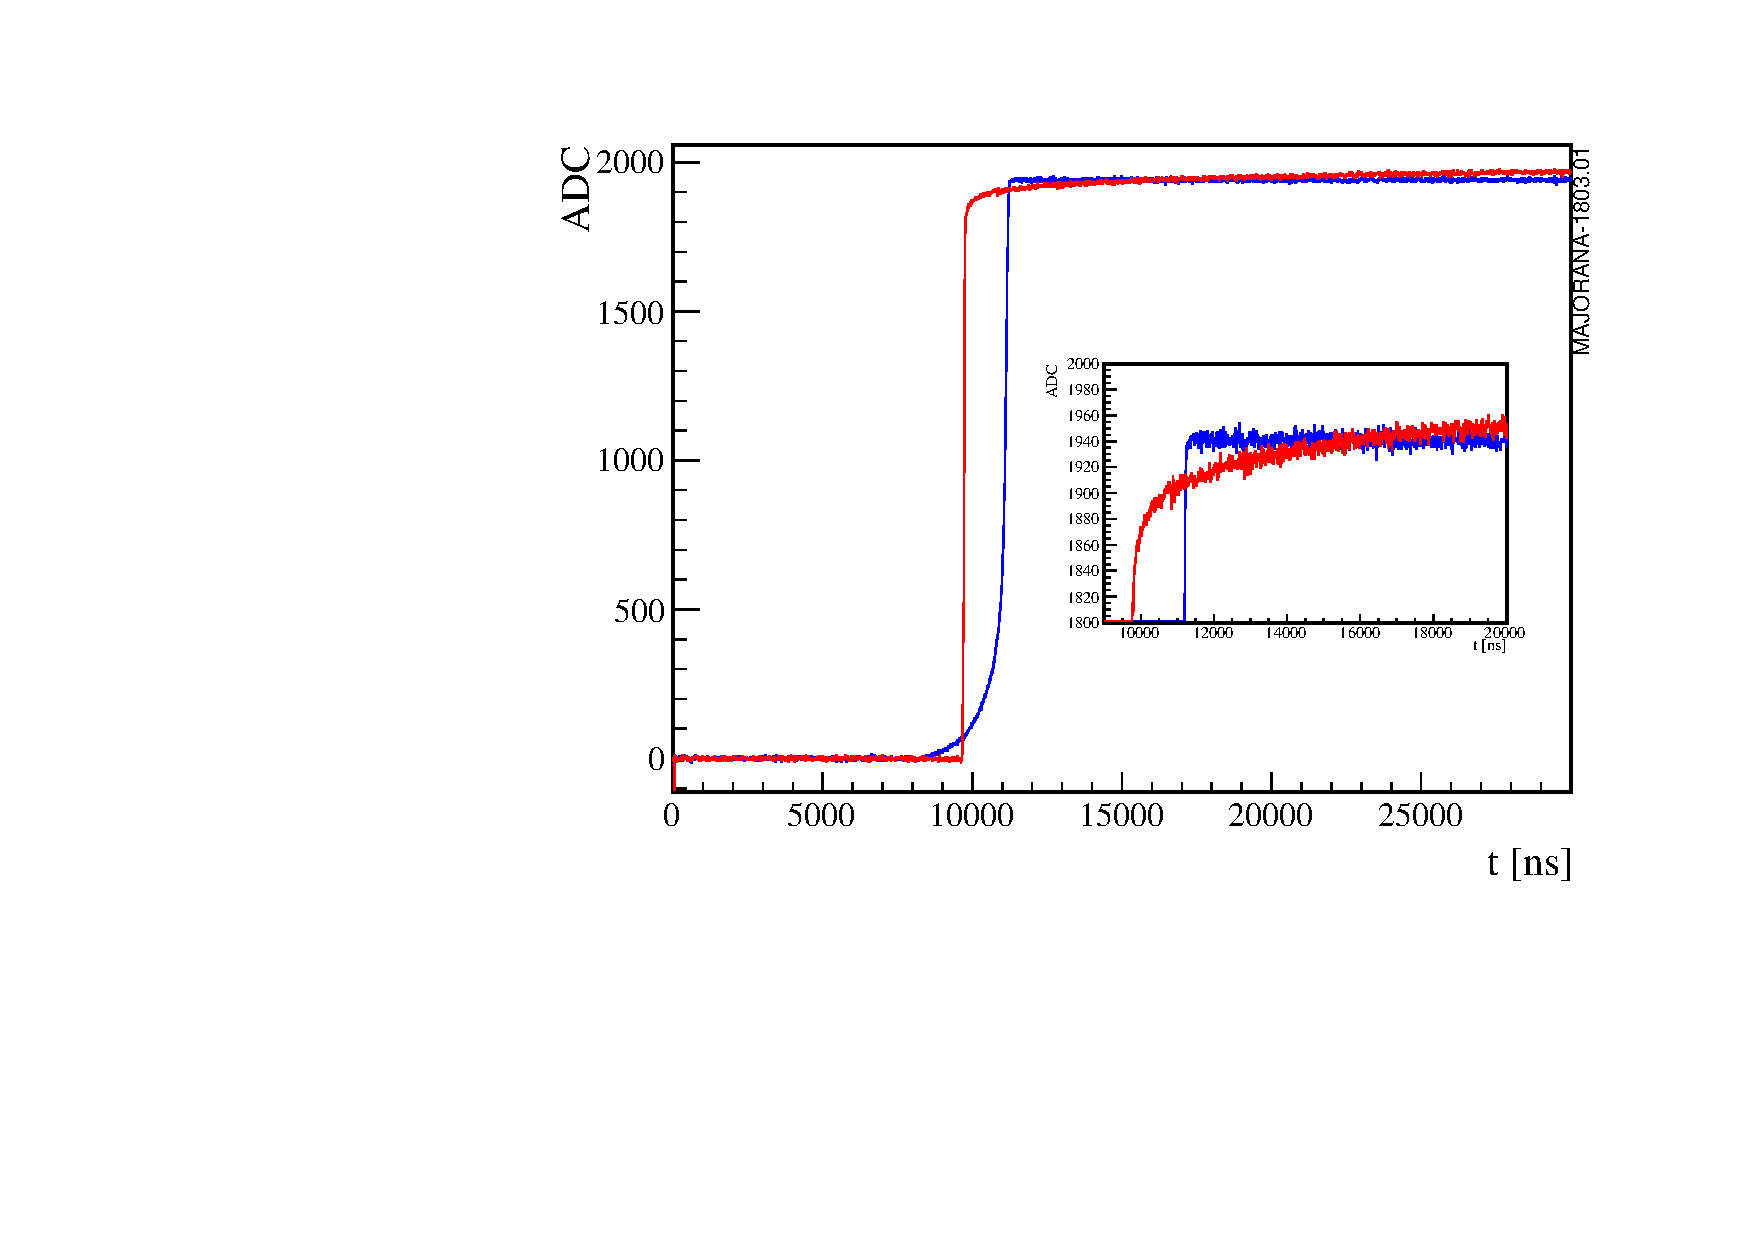
\includegraphics[width=0.6\linewidth]{ch3/figs/dcr_waveform.pdf}
%   \caption{An alpha waveform (red) compared to a bulk waveform (blue) in MJD PPC detector. The slow components result in a distinct tail with a smaller slope, as shown by the highlight area in the box.}
% \label{fig:dcr_waveform}
%   \end{figure}
  
%  This Delayed Charge Recovery (DCR) effect results in energy degradation in the alpha signal. Even though alphas are normally deposited with $5$ MeV energy, the DCR effect leads alphas to potentially contribute to the ROI. For PPC detectors, this could be understood by looking at MJD's energy spectrum, as shown at the top of Fig. \ref{fig:mjd_alpha}. The bottom plot is the difference that highlights alpha contribution in the energy spectrum. The alpha energy spectrum peaks very close to the ROI, which makes it vital to understand how to effectively model and cut alpha events. Creating a background model component for alphas needs accurate modeling of charge collection. Pulse-shaped simulations can help accurately model charge collection and build a background model for alphas.

%  \begin{figure}[htb]
% \centering
%   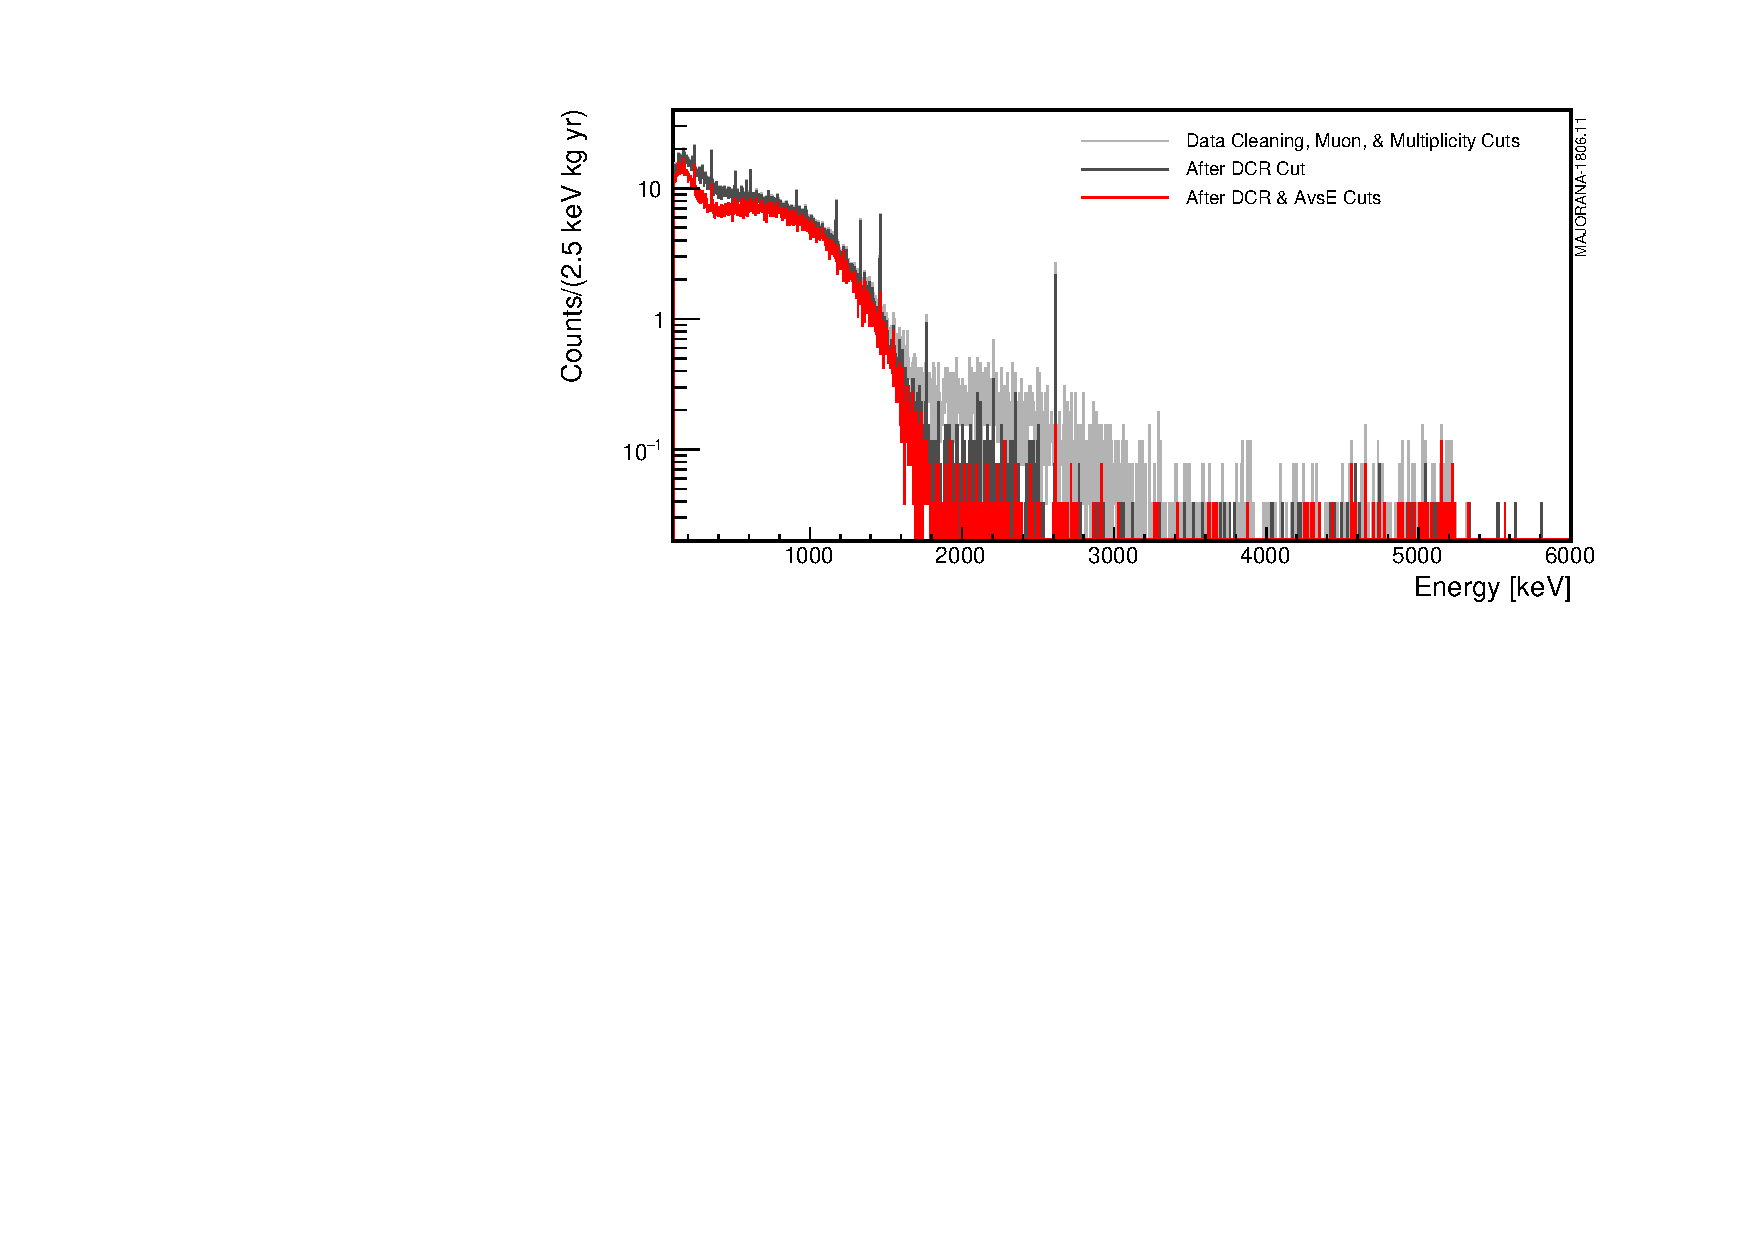
\includegraphics[width=0.8\linewidth]{ch3/figs/mjd_alpha.pdf}
% 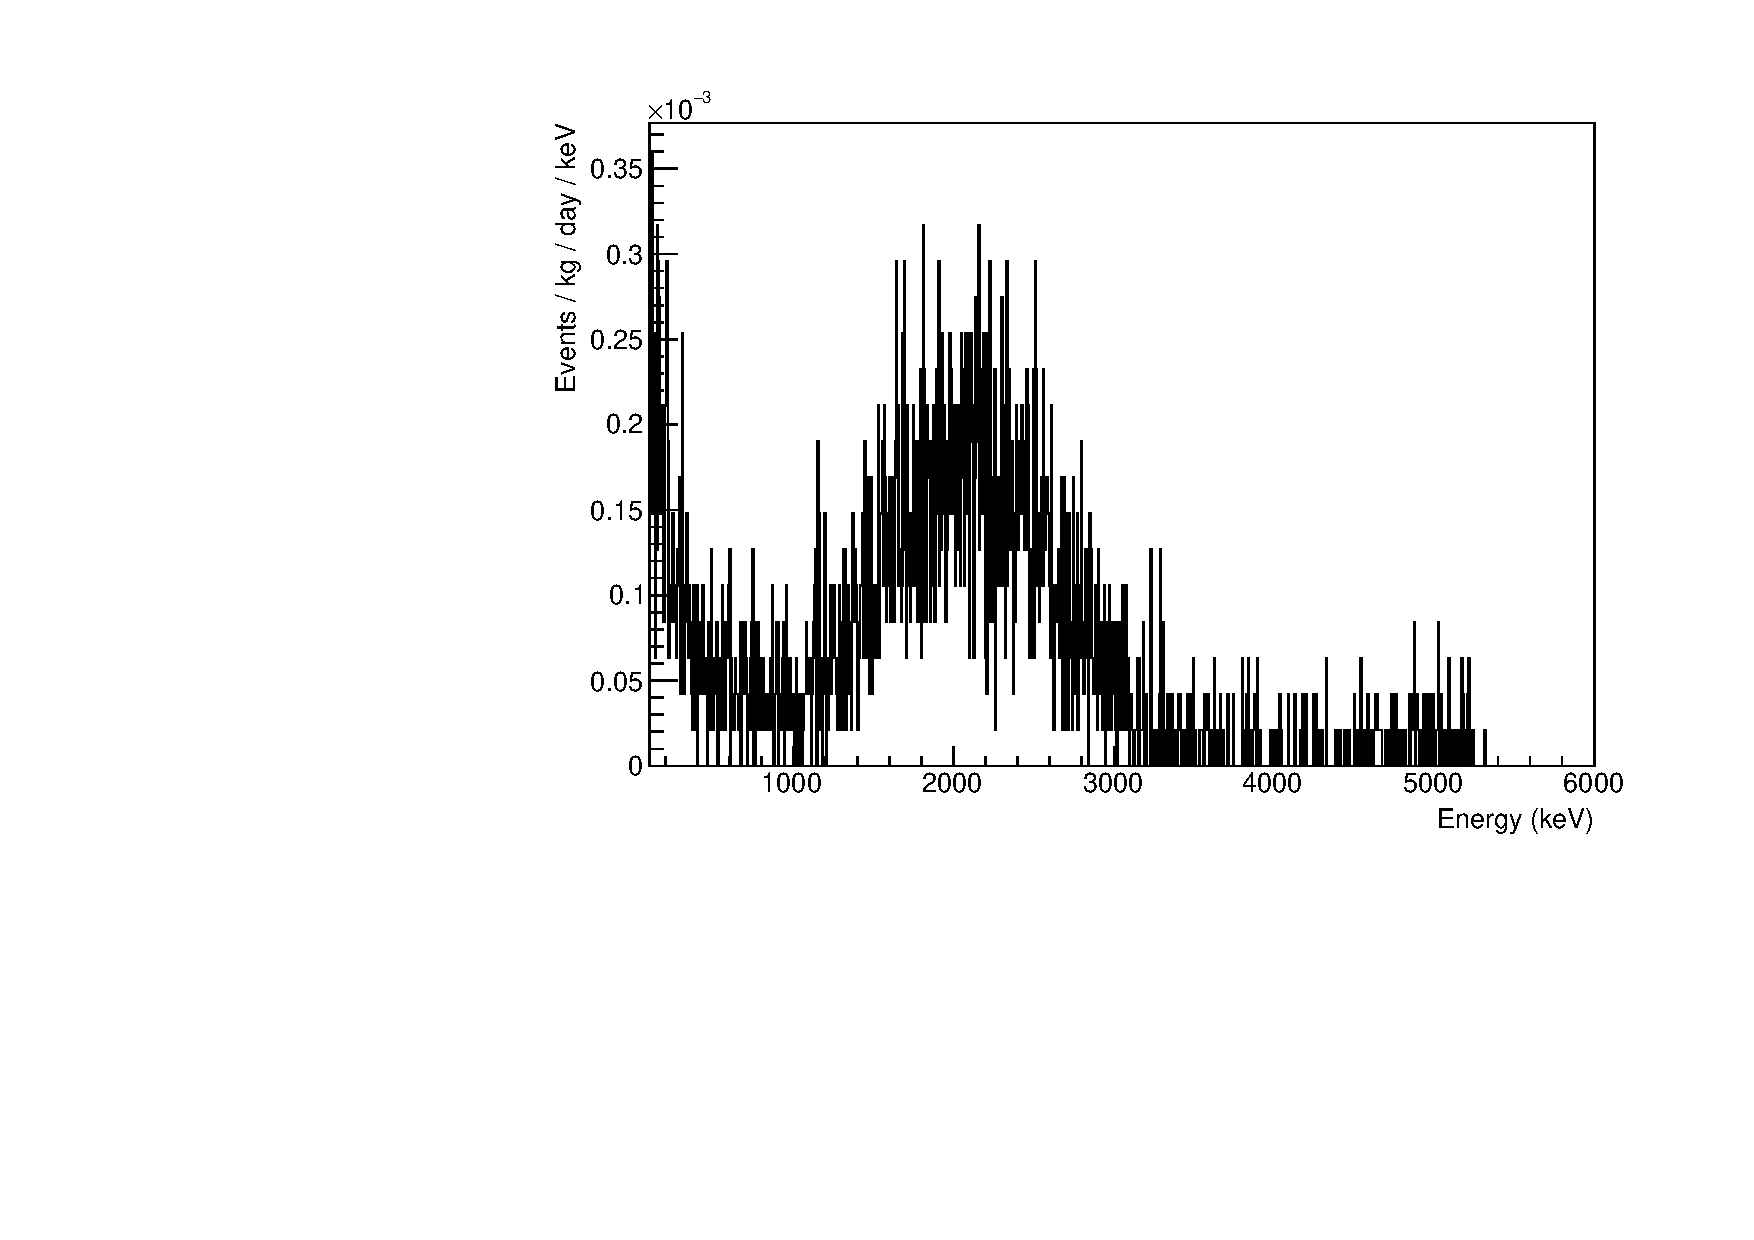
\includegraphics[width=0.5\linewidth]{ch3/figs/MJD_alpha_spec.pdf}
%   \caption{Top: MJD energy spectrum. The light grey line are the events after data cleaning, Muon and multiplicity cuts, and the grey lines are after DCR cuts that remove alpha events. Bottom: The alpha energy spectrum in MJD calculated using the events before and after the DCR cut.}
% \label{fig:mjd_alpha}
%   \end{figure}

\section{Challenges in modelling surface events}
An alpha particle deposits energy of about $4$ - $6$ MeV with a penetration depth of about $17.6$ - $20.0$ micron \cite{knoll_2010}. This excites a lot of charge carriers and produces a dense charge cloud. In such cases, effects such as diffusion of the charges and self-repulsion among charges become significant. Self-repulsion could also push the charge onto the passivated surface, leading to a slower drift and longer collection time for these charges. This slow drift is thought to be due to a combination of charge trapping and re-release near the passivated surface, and slower drift speeds due to surface properties \cite{MULLOWNEY201233}. The passivated surface could also carry a static charge, which could affect the charge collection. In experimental data, these effects manifest as an energy-degraded alpha waveform with a slow rising tail, as shown in Fig. \ref{fig:dcr_waveform}. This Delayed Charge Recovery (DCR) effect degrades the alpha energy spectrum, potentially contributing to the ROI. This underscores the importance of modeling alpha background as alpha events in ROI need to be rejected to have a low background. 

\begin{figure}[!htb]
\centering
  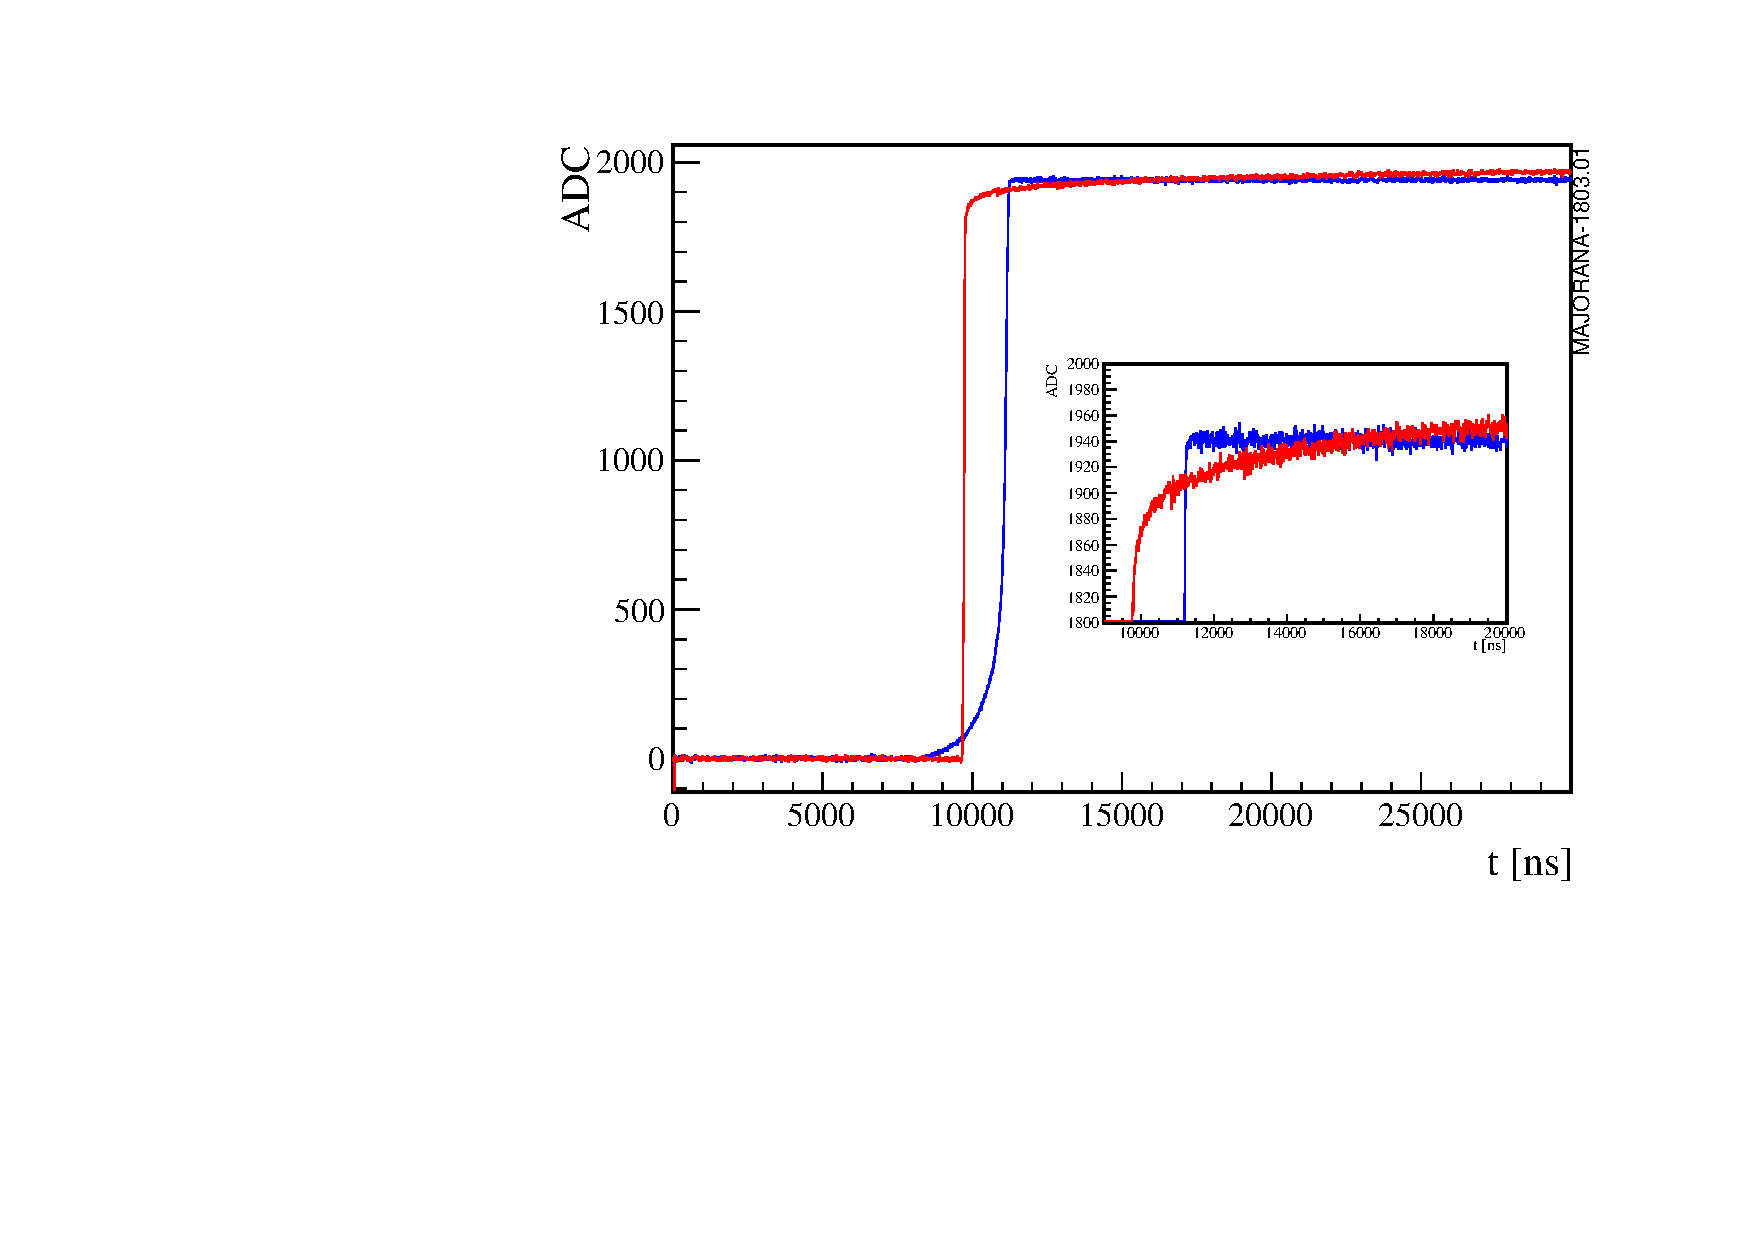
\includegraphics[width=0.95\linewidth]{ch3/figs/dcr_waveform.pdf}
 \caption{An alpha waveform (red) compared to a bulk waveform (blue) in the MJD PPC detector. The DCR effect results in a distinct tail with a smaller slope, as shown by the highlight area in the box.\cite{tube_paper}}
\label{fig:dcr_waveform}
  \end{figure}

Pulse shape simulations provide a way to perform alpha background modeling since signal formation in Germanium is well understood. A simulation to model alphas should allow for a nonspherical charge cloud while incorporating surface drift, diffusion, and self-repulsion. This warrants a dedicated simulation for surface alphas.


\begin{figure}[!htb]
\centering
  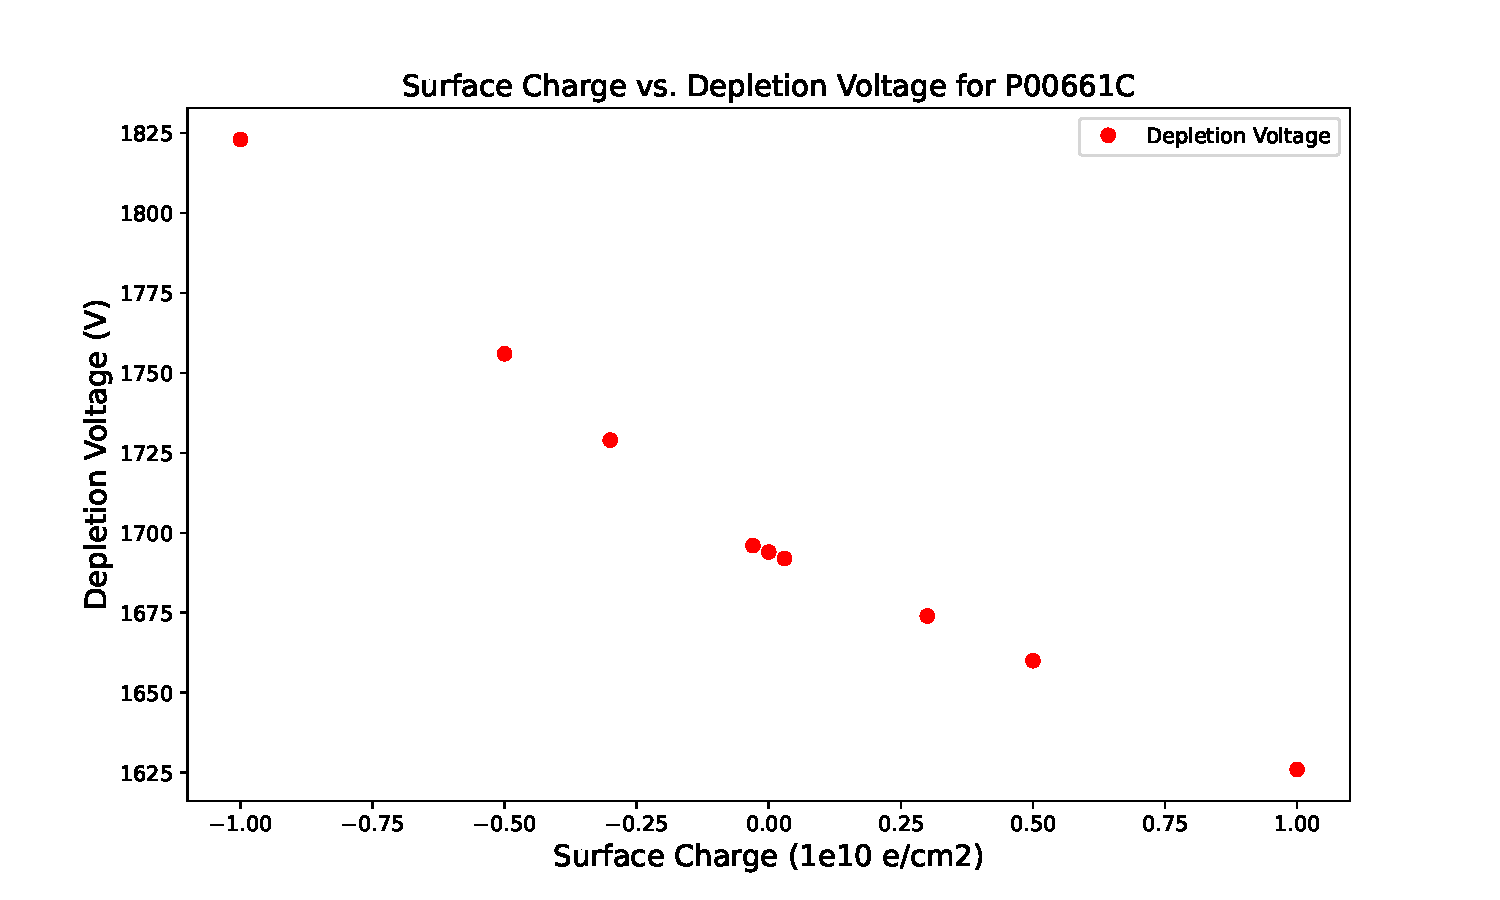
\includegraphics[width=0.99\linewidth]{ch3/figs/deplep_sc.pdf}
 \caption{Effect of surface charge on depletion voltage for LEGEND PPC detector.}
\label{ch3:fig:deplection_sc}
  \end{figure}
Simulations within the LEGEND collaboration include Siggen \cite{siggen_paper} and SSD simulations \cite{Abt:2021SSD}.

\section{Pulse shape simulations till now}

Signal formation in Germanium is well understood via the Shockley-Ramo theorem. This enables building accurate simulations that can model the waveforms. Simulations within the LEGEND collaboration include Siggen and SSD simulations. 

Siggen is a C-based program initially developed by David Radford at Oak Ridge National Lab for MJD pulse shape simulations \cite{siggen_paper}. It consists of two components: fieldgen and siggen. Fieldgen is used to calculate the electric potential and weighting potential of point-contact detectors in two-dimensional cylindrical coordinates. The siggen part uses the weighing potential calculated from fieldgen to generate a signal. The simulations can calculate the depletion voltage, the volume of the depletion region, and the capacitance of the detector. Diffusion in siggen is approximated using a Gaussian convolution, and there is no mechanism to account for the self-repulsion of charges as Siggen uses point charges to represent the entire charge cloud.

% A simulated event in Siggen is shown in Fig. \ref{fig:siggen_1d}.

% \begin{figure}
% \centering
% 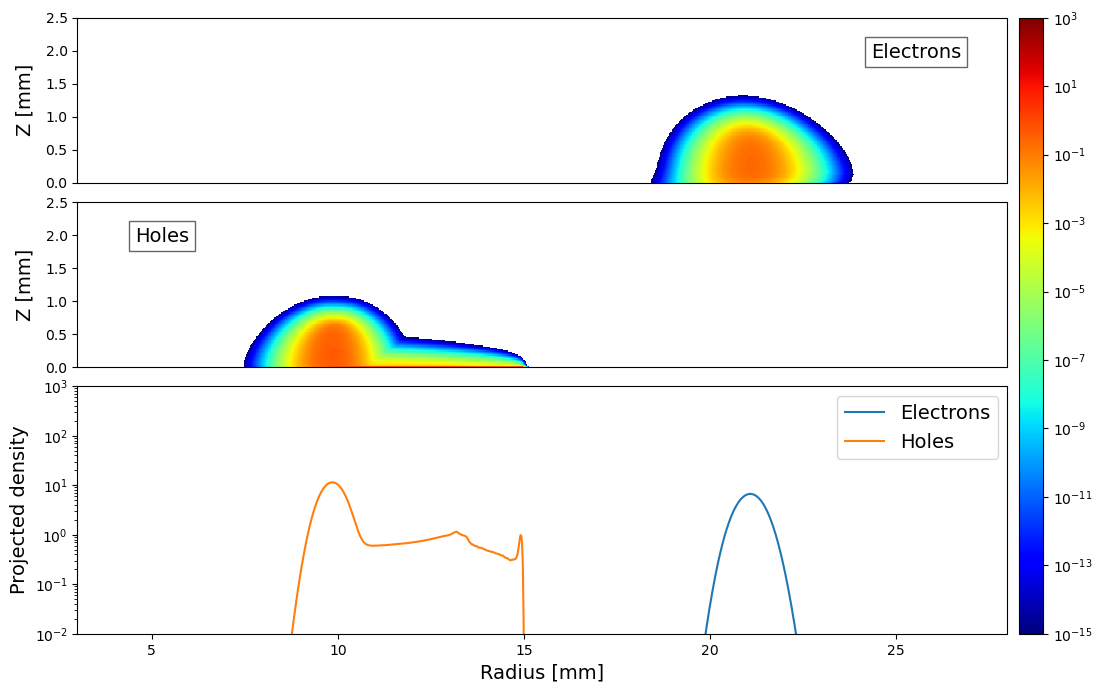
\includegraphics[width=0.49\linewidth]{ch3/figs/drift_path.png}
% 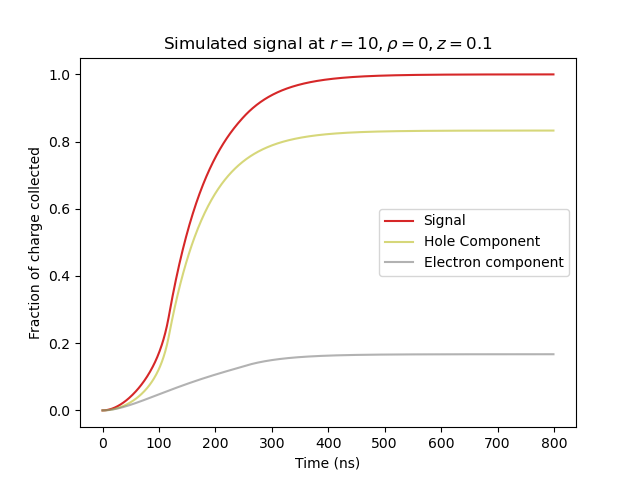
\includegraphics[width=0.49\linewidth]{ch3/figs/samp_wav_comp.png}
% \caption{A simulated event showing the path of holes and electrons and the corresponding waveform}.
% \label{fig:siggen_1d}
% \end{figure}

SolidStateDetectors.jl (SSD) is a software package developed by the group of Iris Abt at the Max Planck Institute Munich for the LEGEND experiment \cite{Abt:2021SSD}. It is written in Julia and can perform calculations in all 3 dimensions. SSD can calculate electric fields and potentials outside the detectors and has the ability for parallelization. The SSD enables full 3D diffusion and model self-repulsion in the signal. The charges are tracked individually using their position and velocity.

In bulk, a spherical charge cloud model works very well, but the charge cloud produced by alpha is not necessarily spherical due to the charge trapping and re-release effect on the passivated surface. A simulation to model alpha should allow for a nonspherical charge cloud while incorporating surface drift, diffusion, and self-repulsion.

% \begin{figure}
% \centering
% 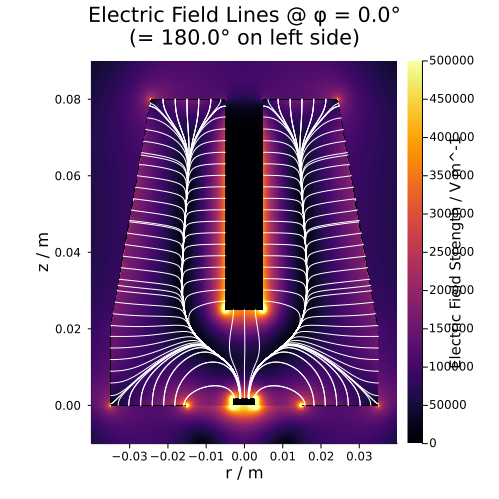
\includegraphics[width=0.49\linewidth]{ch3/figs/ssd_e.png}
% 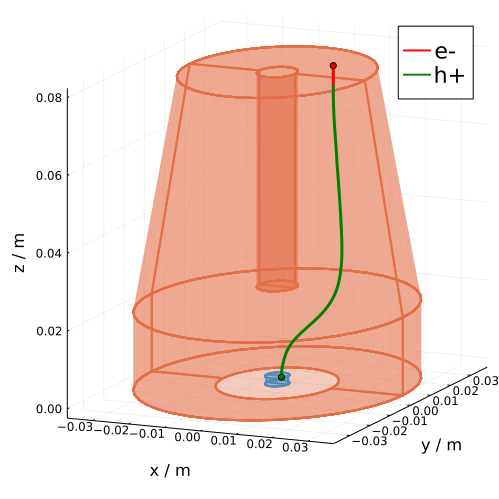
\includegraphics[width=0.49\linewidth]{ch3/figs/ssd_path.png}
% \caption{Simulated Electric field and charge paths in SSD simulations. It allows for calculations outside the detectors and in full 3 dimensions. \cite{ssd_web}.}
% \label{fig:ssd_plots}
% \end{figure}


\section{{\tdsim}}

{\tdsim} are new methods to simulate surface alpha events while directly simulating diffusion and self-repulsion effects. They were initially programmed in C by David Radford and build upon Siggen simulations developed for MJD \cite{siggen_paper}. As charges drift through the detectors, they keeps track of charge densities at a pixel-by-pixel level, which allows for nonspherical charge clouds. The charges that end up on the surface have their velocities reduced by a predetermined factor. {\tdsim} also enables simulation of the effects of surface charges. The simulation is performed in r and z-direction while assuming $\phi$ symmetry— thus the charge cloud is simulated by a ring. Diffusion is performed in 2D, but the diffusion speed was checked against the diffusion speed of 3D charge clouds. The simulations need a fine grid size to account for the low penetration depth of surface alphas. The charges that end up on the surface have their velocities reduced by a predetermined factor. {\tdsim} also enables simulation of the effects of surface charges.


Fig. \ref{fig:ehd_flowchart} shows how the {\tdsim} program works. The detector is divided into a grid, and charge densities are distributed at a given location based on the impact energy, usually over two adjacent grid points. The boundary conditions are set according to the detector geometry, impurity concentration, surface charge, and bias voltage. Then electric potential and weighting potential are calculated using an over-relaxation algorithm. The capacitance and depletion are estimated. Undepleted regions of a semiconductor detector have no net space charge and no electric field and are indicated by a local minimum in the electrical potential. The capacitance is calculated by relating two equations for the energy stored in a capacitor.

\begin{equation}\label{capacitance_eq}
C= \frac{\epsilon}{V^2} \int_{}^{} E^2 dA
\end{equation}

\begin{figure}
\centering
%[trim={left bottom right top},clip]
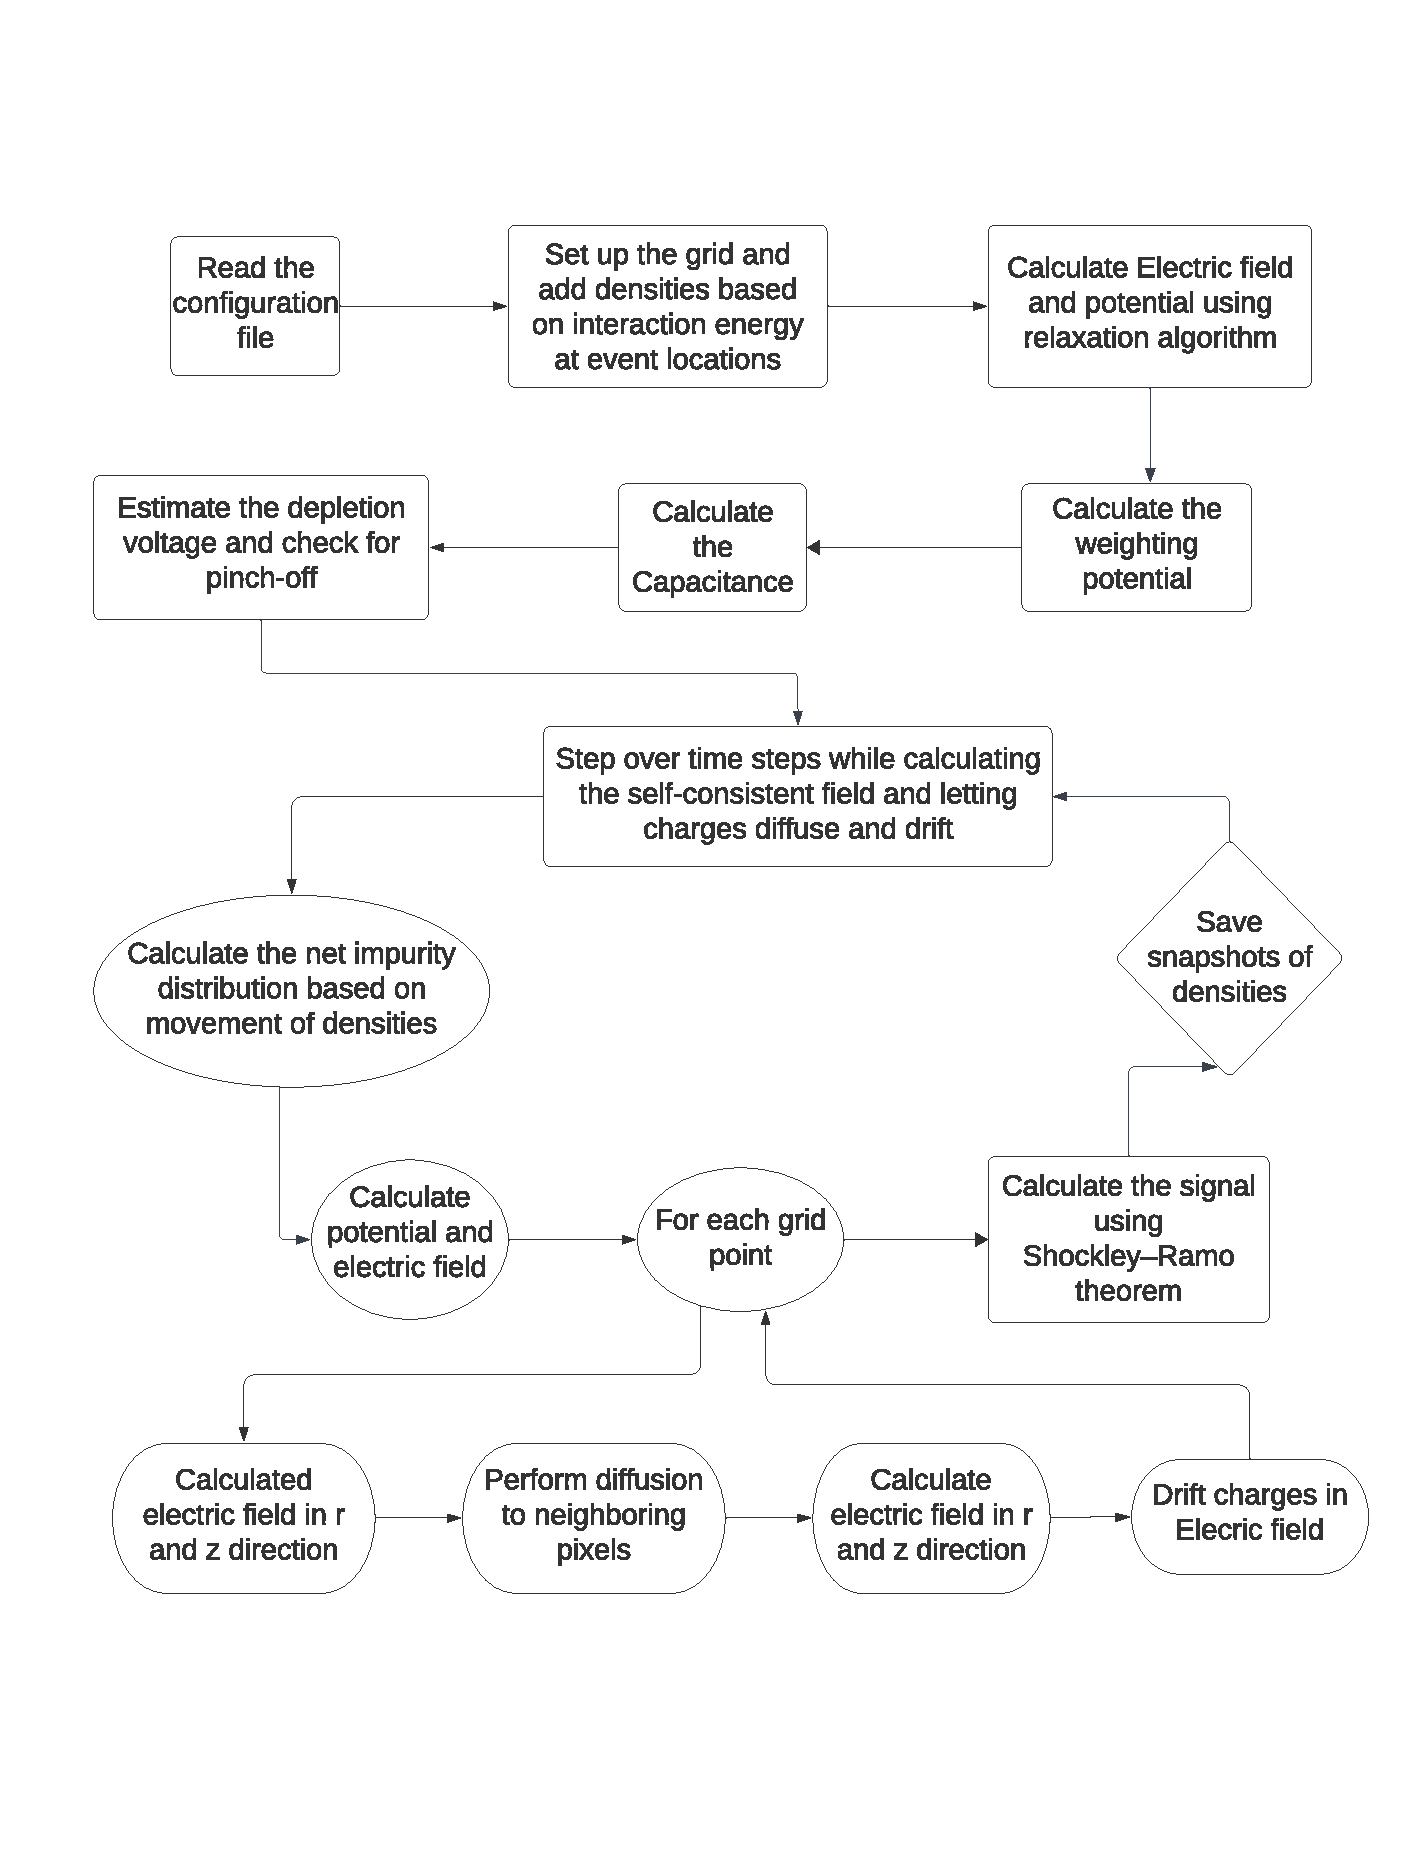
\includegraphics[width=0.99\linewidth,trim={2pc 10pc 1.5pc 9pc},clip]{ch3/figs/ehd_flowchart.pdf}
\caption{A flow chat illustration the pseudo code for {\tdsim}.}
\label{fig:ehd_flowchart}
\end{figure}

After the initial setup, the program steps through a small time step. The charges are allowed to diffuse using Einstein's diffusion equation and then drift in the electric field. The net impurity distribution is updated based on the movement of these charges. The electric potential is recalculated based on the new net impurity distribution to account for the fact that the movement of a large charge cloud can change the field inside the detector. Charges that end up on the surface drift slowly based on an input speed. The charge density at each location is saved to a file at regular intervals. These files are read later to generate a signal.

\section{Diffusion}
\begin{equation}
    D = \frac{\mu k_B T}{q} ,
\end{equation}

Fig. \ref{ch3:fig:ehd_path_pd_sc0} shows a snapshot at time=$80$ns of the electron and hole clouds drift in the {\tdsim} for a 5 MeV energy deposition close to the surface with no charge. The projected density shows the distribution of the charge in the cloud. The head of each signal has a peak which is where charges would have normally traveled in point charge simulations. The tail of the projected density has a peak that is due to the slow drift of the charges on the surface. The drift on the surface, in this case, is set to be $1000$ slower than drift in bulk. This matches the range of possible effects found in \cite{MULLOWNEY201233}. 

-equation for initial cloud size
-how surface driftr works

{\tdsim} also provides several custom tunable parameters such surface charge, surface to bulk drift ration, initial energy, etc. that can be used to match the data. Fig. \ref{fig:wf_comp} shows how the output changed with surface to bulk drift and surface charge. High surface charge means that more charges will be pulled onto the surface and thus less sharp rising part will have lower magnitude. A faster surface to bulk ration means that the charges on the surface will be collected fast and so the tail shape will be different.

\begin{figure}
    %[trim={left bottom right top},clip]
    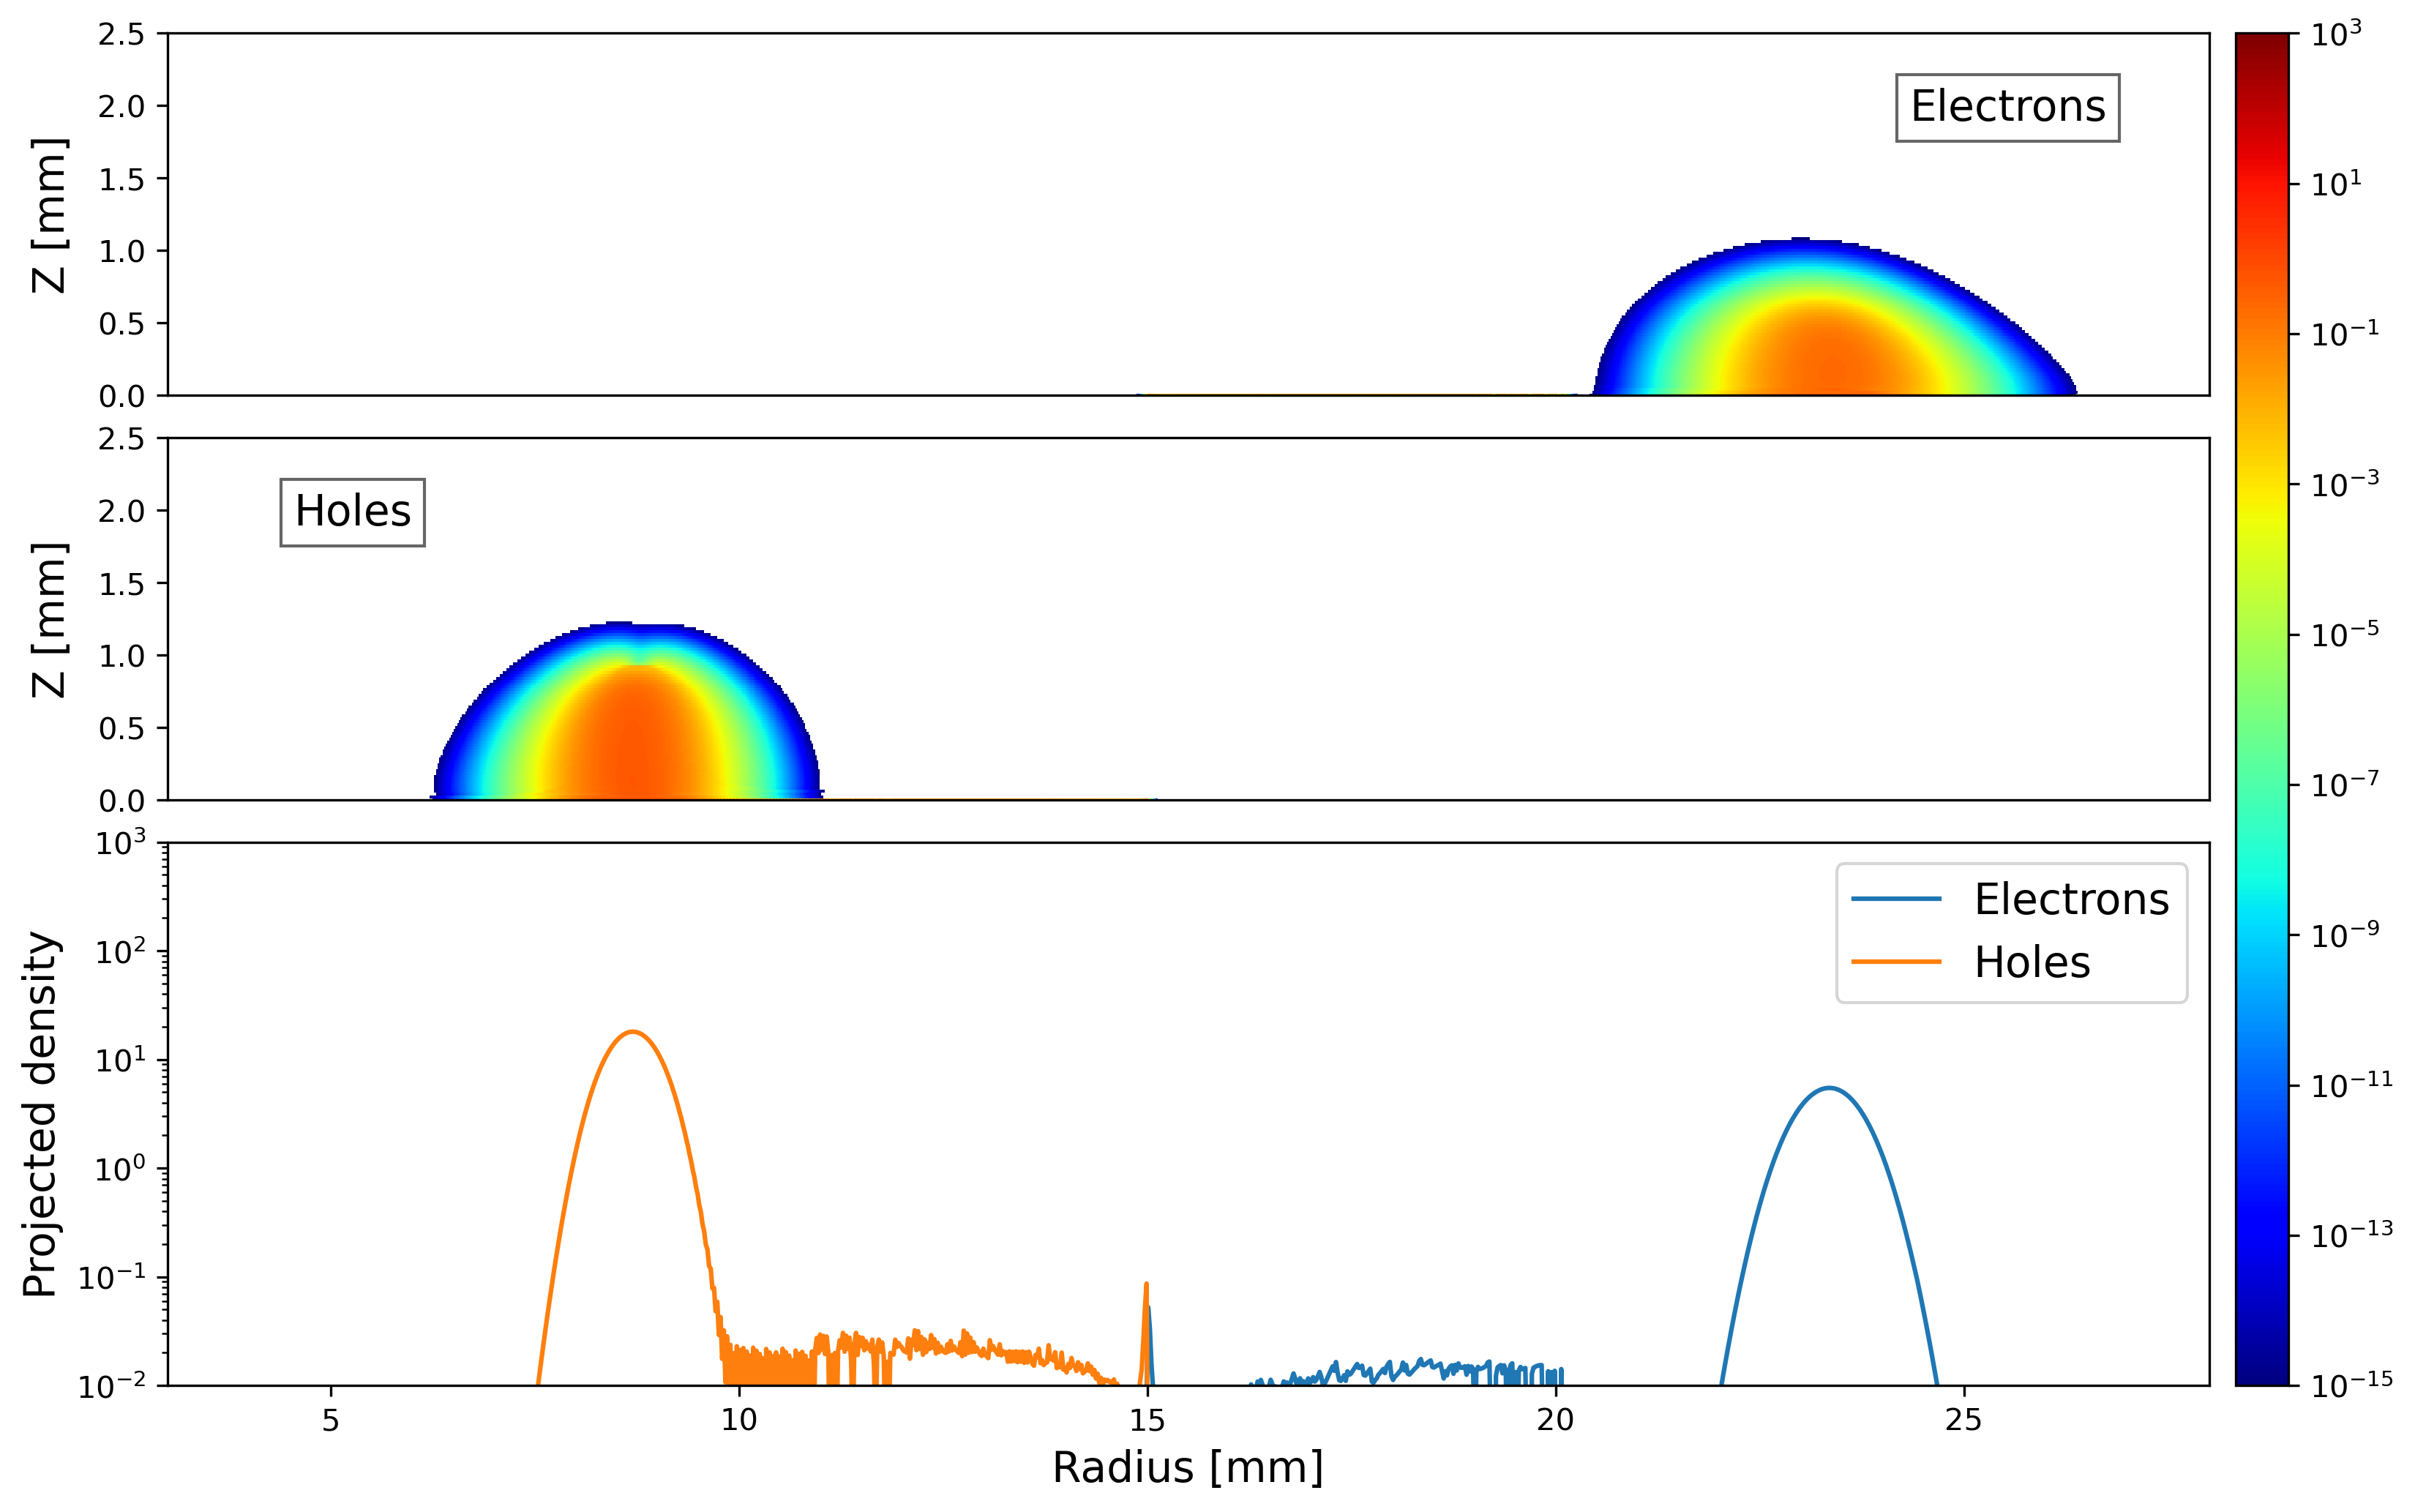
\includegraphics[trim={0cm 0 0cm 0},clip,width=0.99\linewidth]{ch3/figs/drift_path_sc=0.0.png}
    \caption{Drift of electron and hole charge clouds in {\tdsim}. The projected densities show how the charges are distribution along the radius. The density have two peak, one due to fast moving component in bulk and another due to slow moving component on the surface.}
    \label{ch3:fig:ehd_path_pd_sc0}
\end{figure}


\begin{figure}
    %[trim={left bottom right top},clip]
    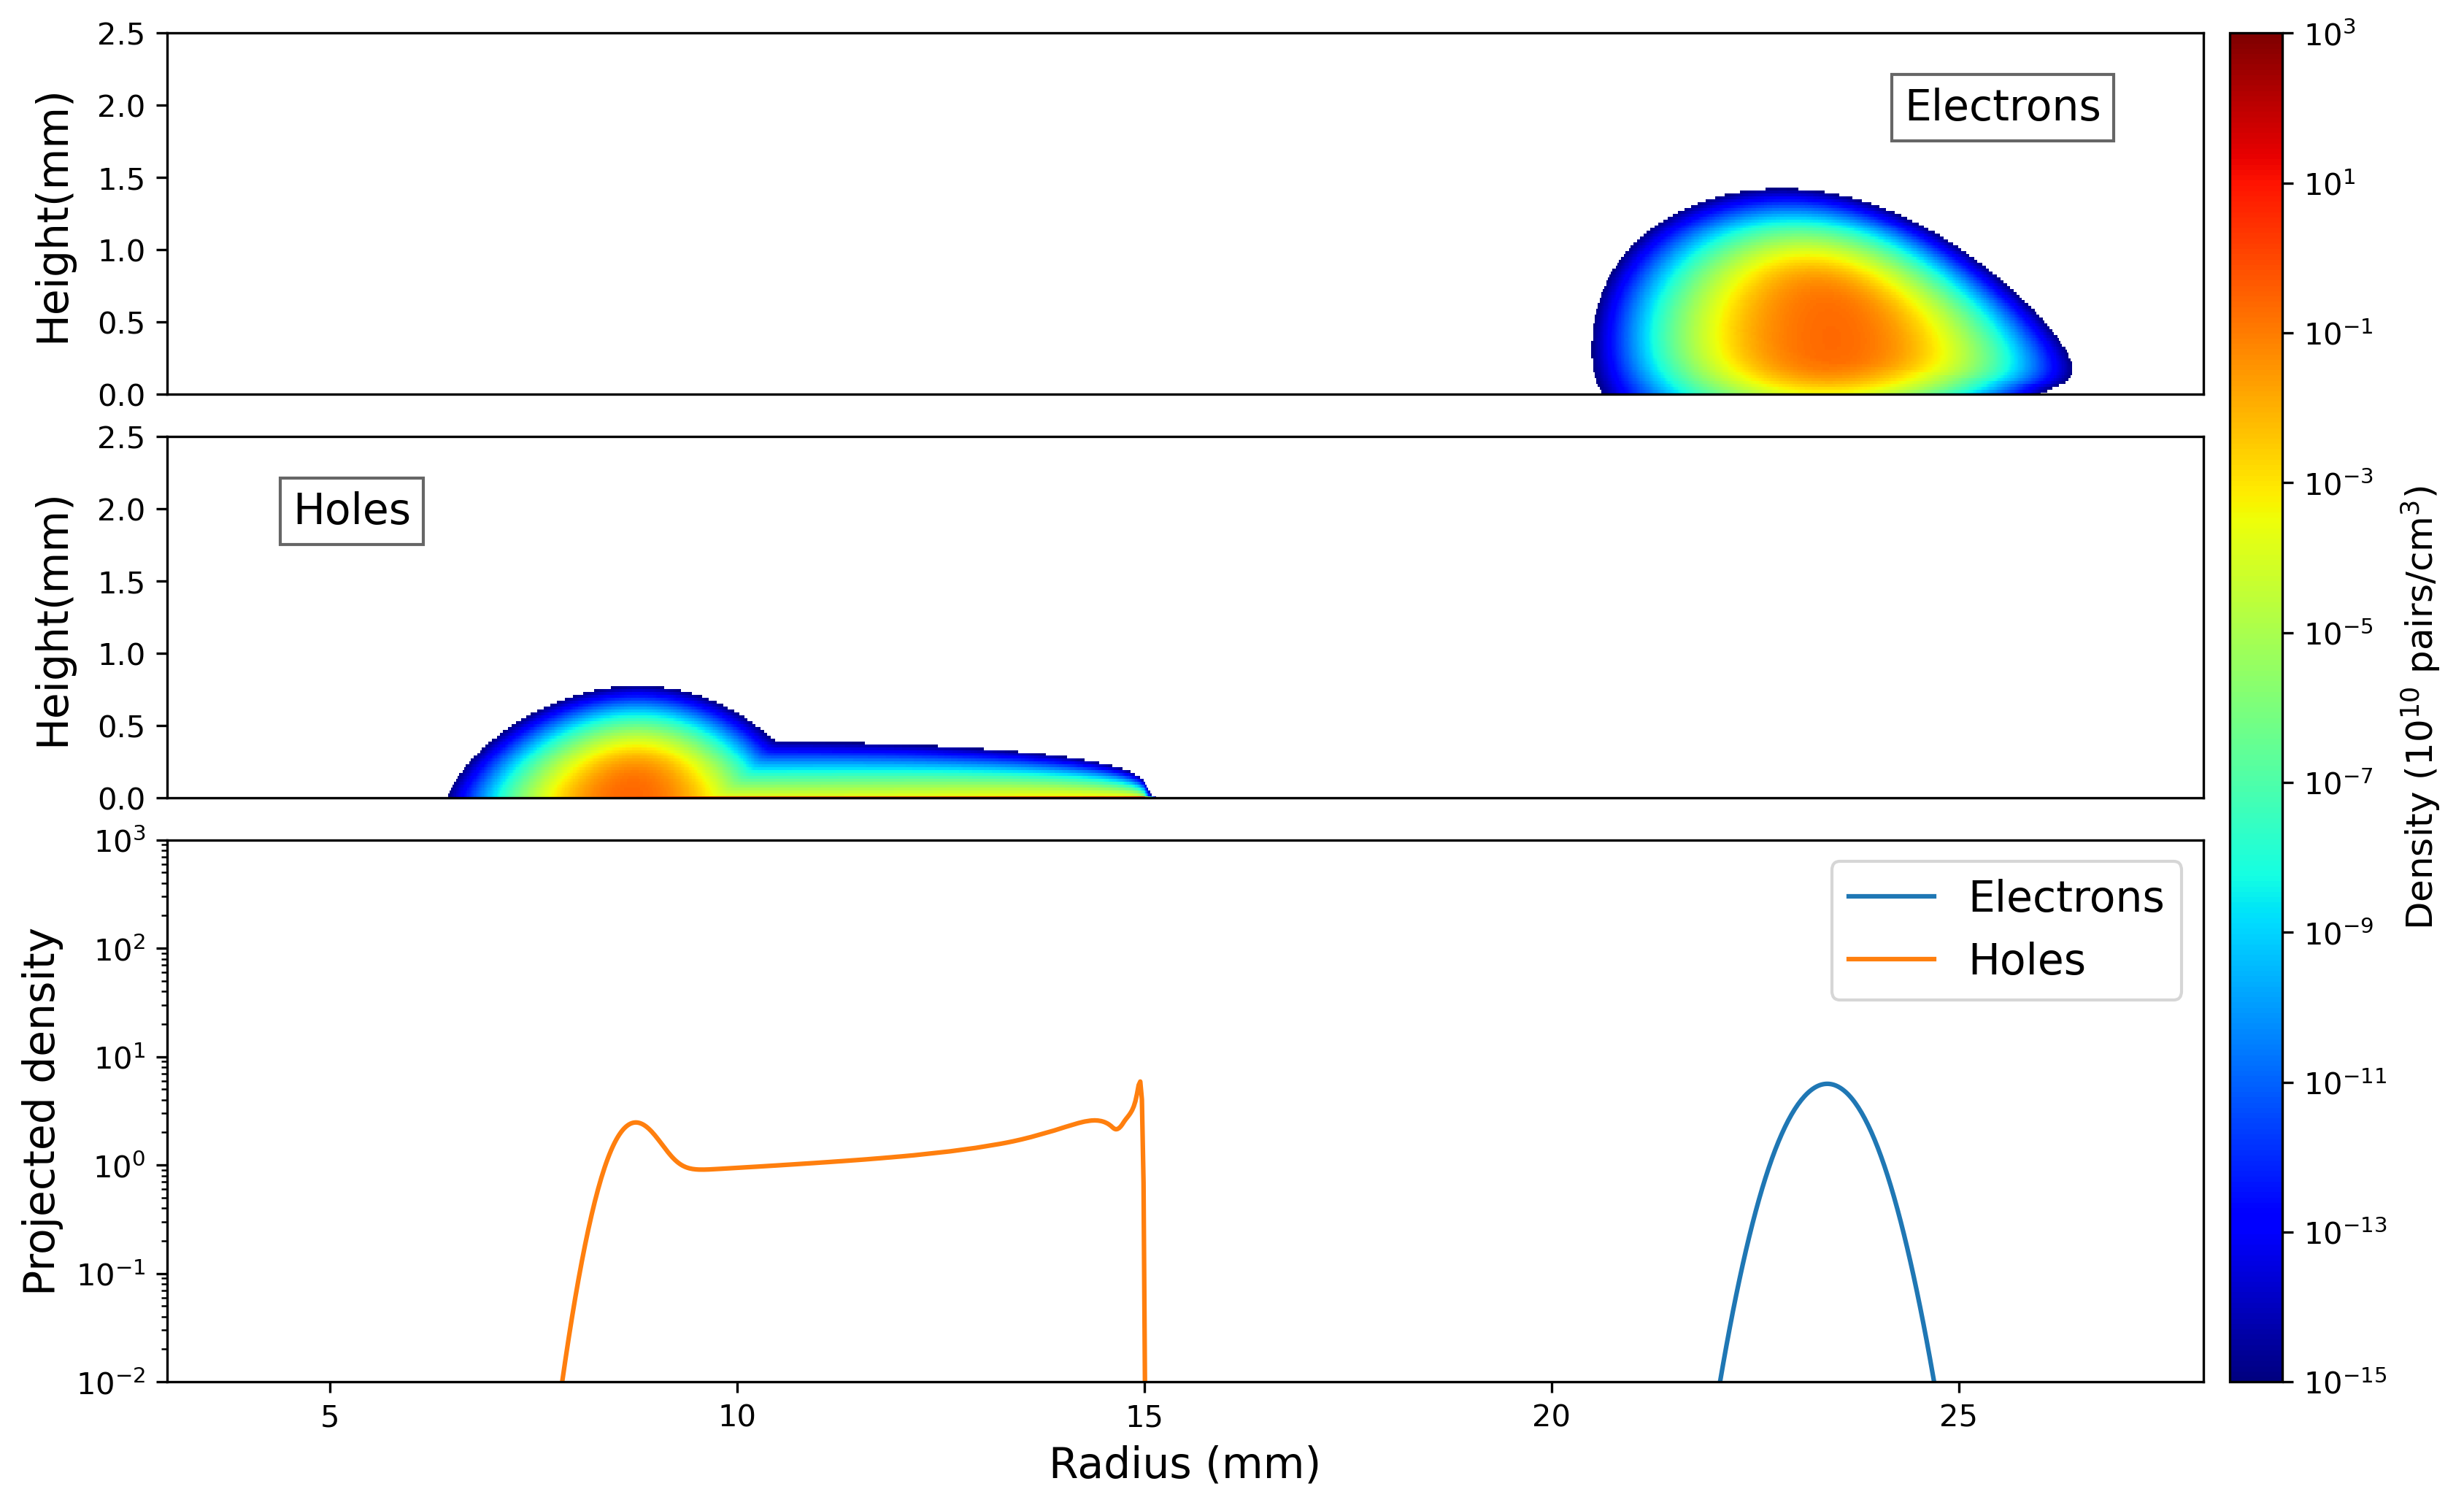
\includegraphics[trim={0cm 0 0cm 0},clip,width=0.99\linewidth]{ch3/figs/drift_path_sc=-0.3.png}
    \caption{Drift of electron and hole charge clouds in {\tdsim}. The negative surface charge pulls the holes onto the surface which move at a slower speed.}
    \label{ch3:fig:ehd_path_pd_sc-0.3}
\end{figure}



\begin{figure}
    %[trim={left bottom right top},clip]
    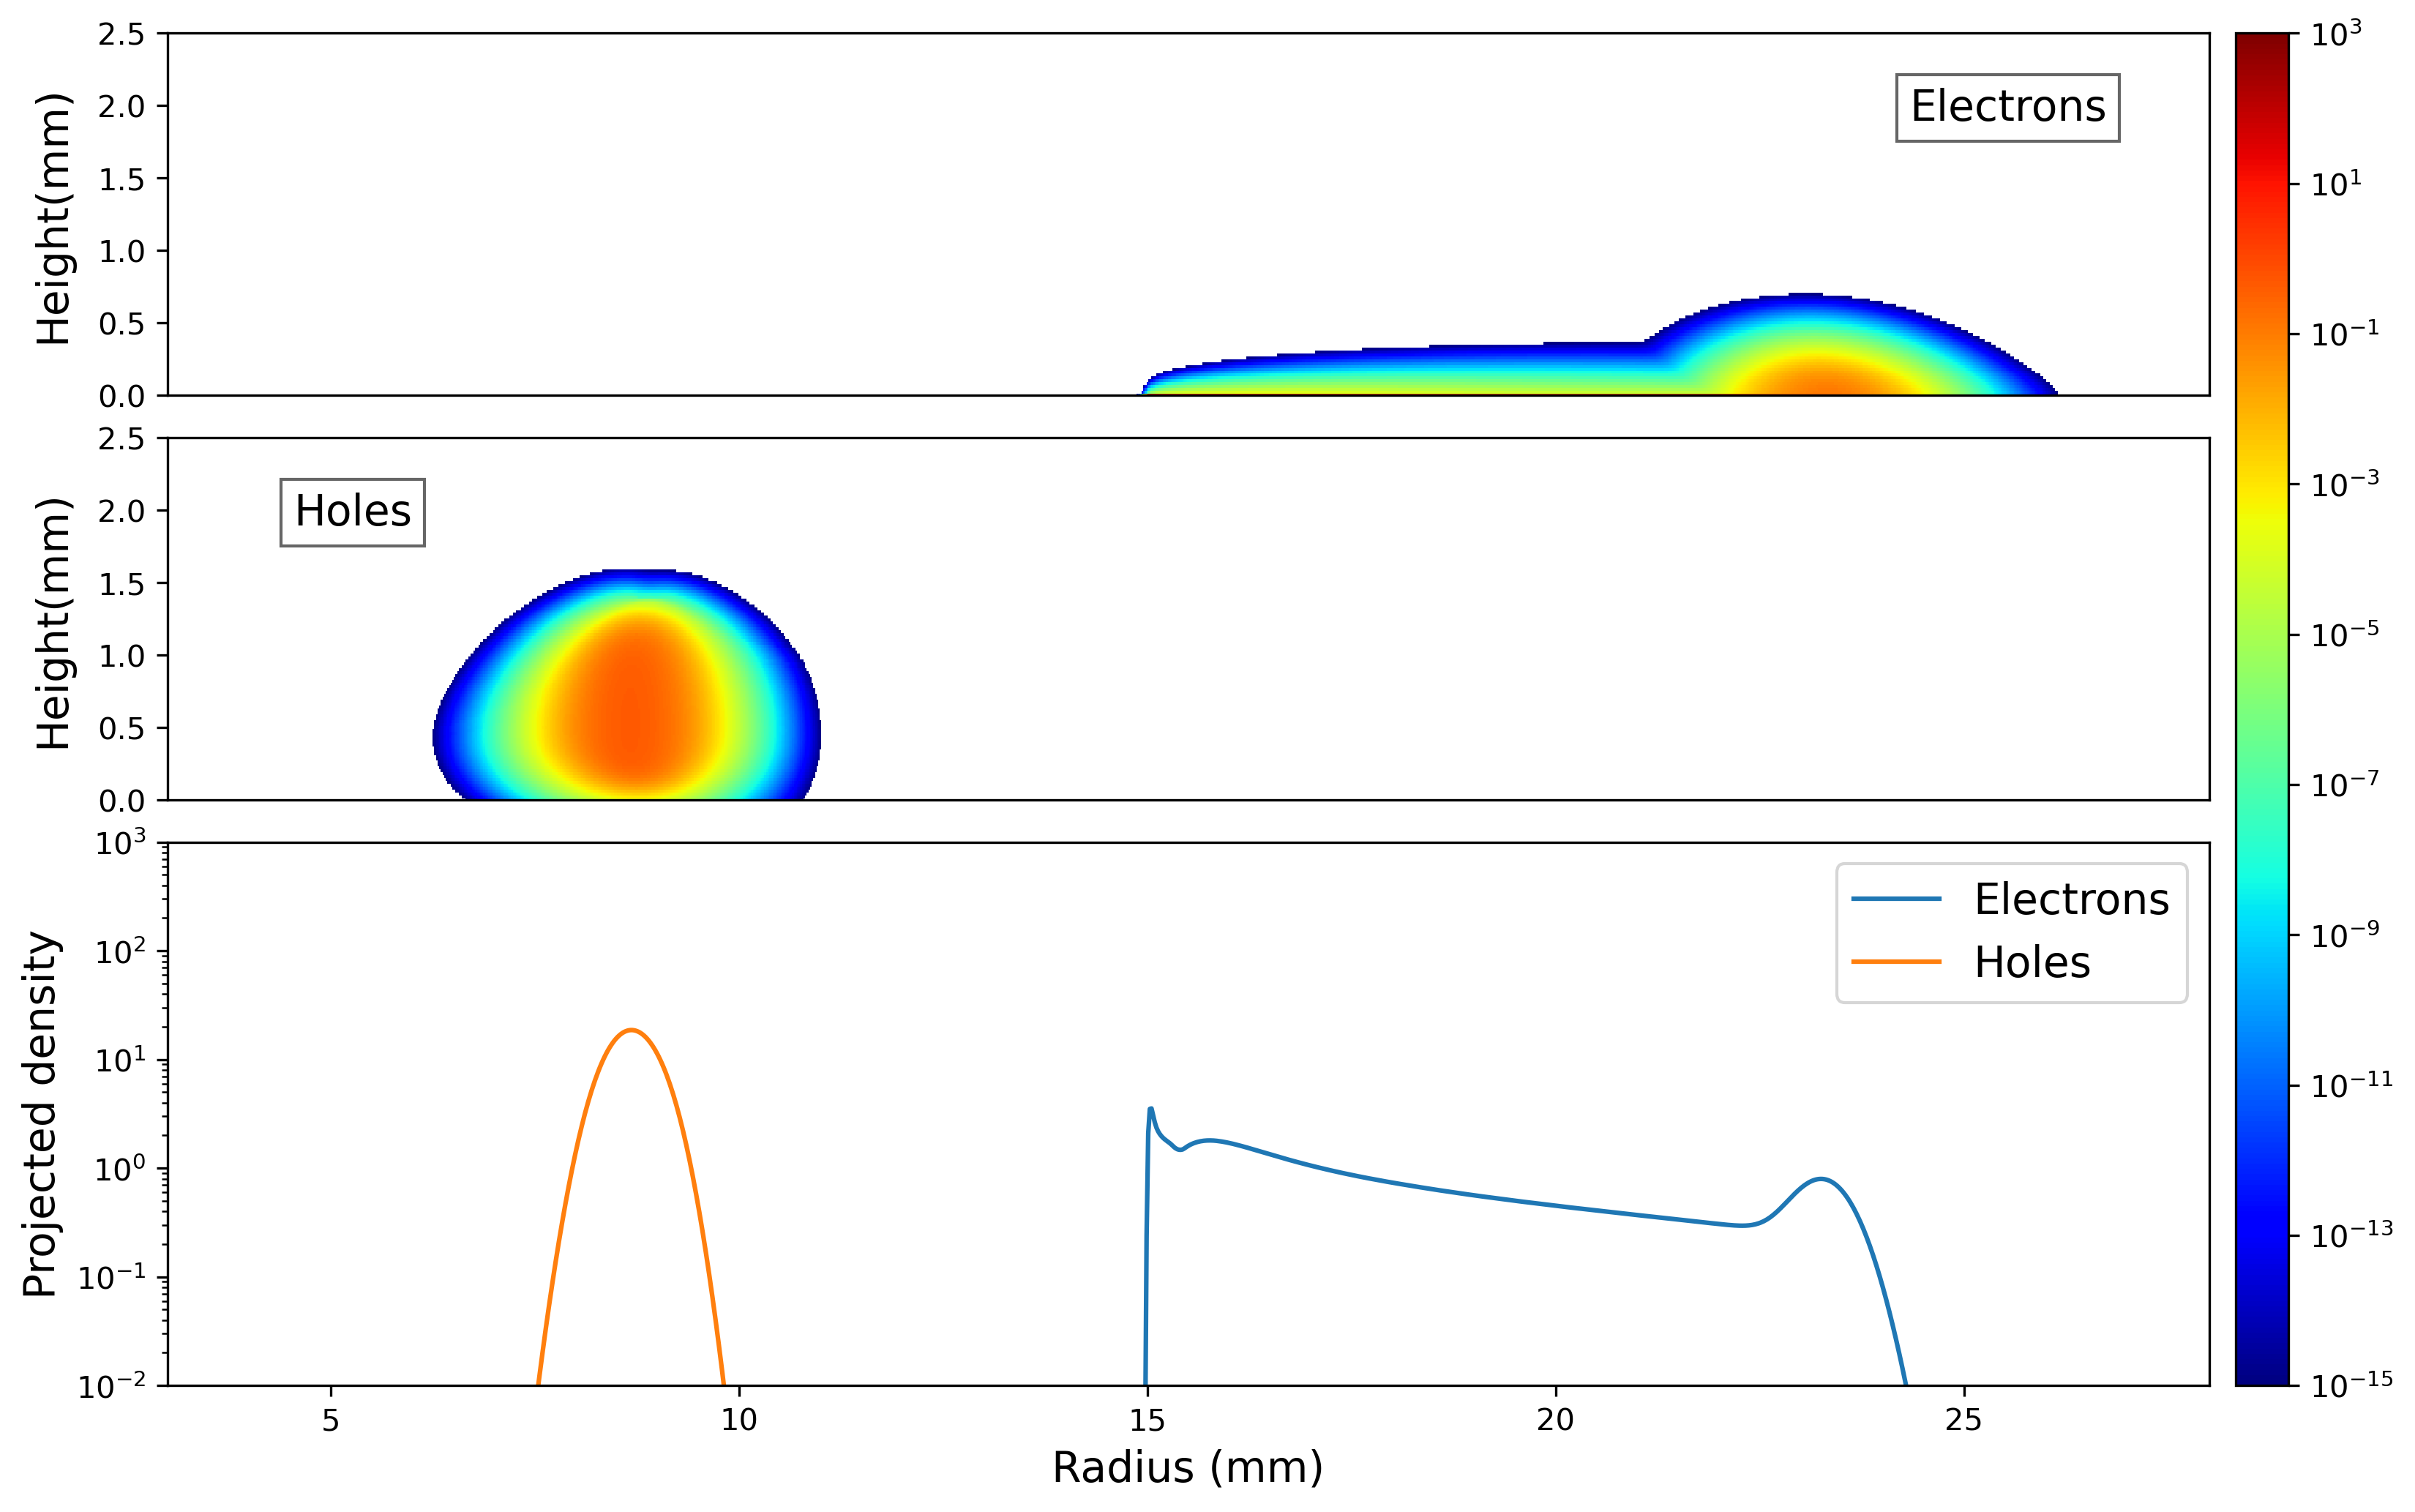
\includegraphics[trim={0cm 0 0cm 0},clip,width=0.99\linewidth]{ch3/figs/drift_path_sc=0.3.png}
    \caption{Drift of electron and hole charge clouds in {\tdsim}. The positive surface charge pulls the electrons onto the surface which move at a slower speed.}
    \label{ch3:fig:ehd_path_pd_sc0.3}
\end{figure}

\begin{figure}
    %[trim={left bottom right top},clip]
    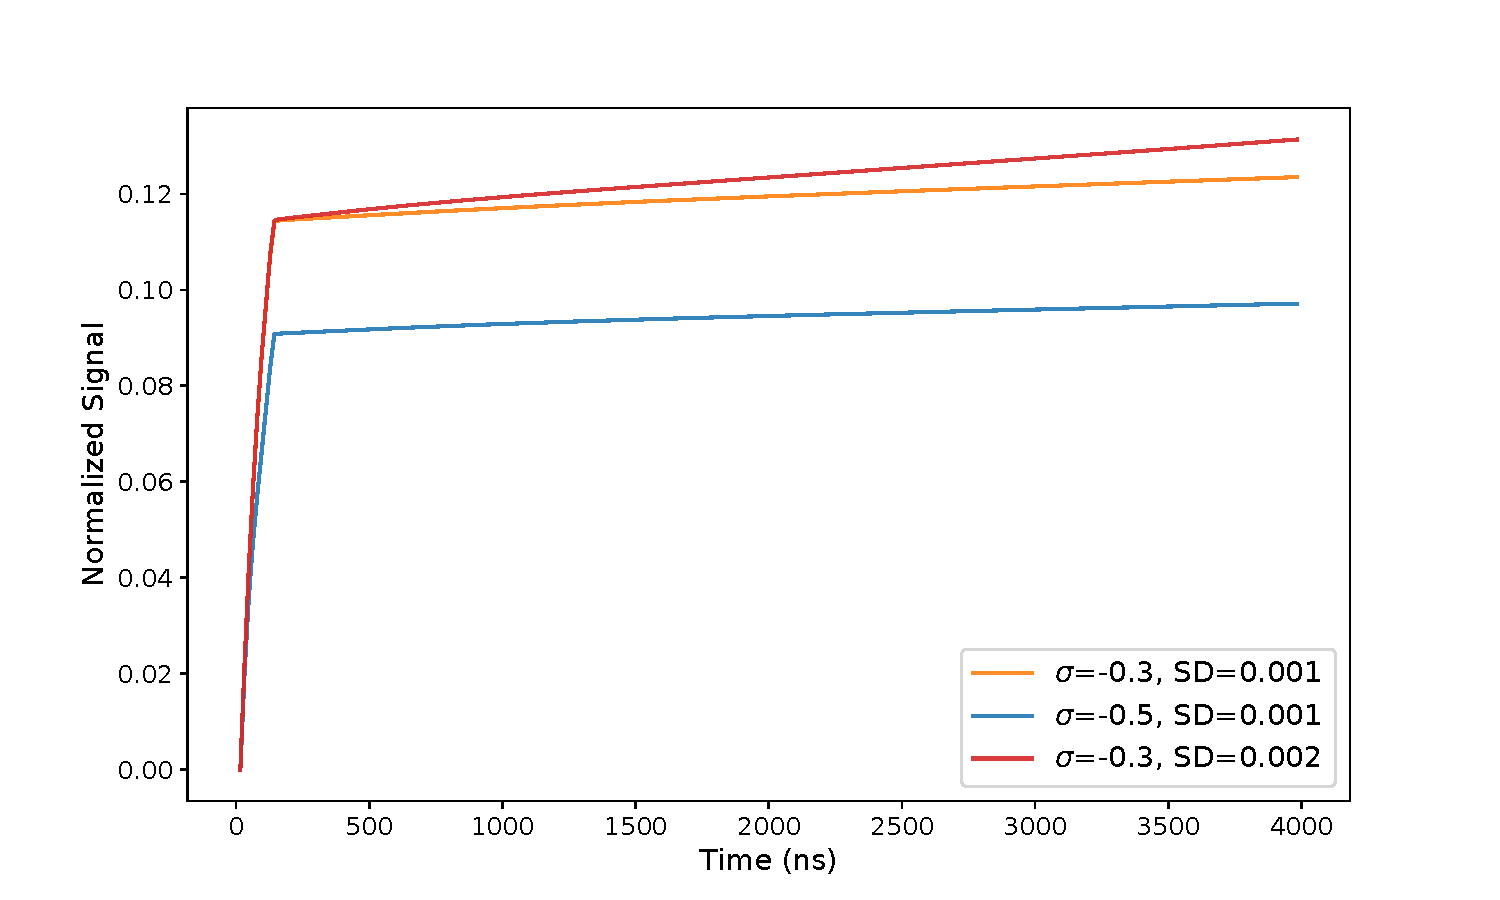
\includegraphics[trim={0.1cm 0.3cm 1.3cm 0.3cm},clip,width=0.99\linewidth]{ch3/figs/wf_comp.pdf}
    \caption{A comparison of waveforms generated by {\tdsim} for a {\Ltwo} PPC detector based of different tunable parameters surface charge ($\sigma$) and relative surface drift velocity (SD).}
    \label{fig:wf_comp}
\end{figure}

The {\tdsim} approach better models surface alpha waveforms by incorporating diffusion, self-repulsion, and field recalculations. However, it is computationally expensive. A simulation of an $800$ns event for a surface alpha event with a $10$-micron grid can take up to $7$ hours to run on a supercomputer cluster. This is primarily because the electric potential has to be recalculated at each time step.


Fig. \ref{fig:GPU_time} shows the run time for the entire program and an initial electric potential calculation. In general, the smaller the grid, the more points to update and the longer the time to run the program. To correctly model alphas backgrounds, a multitude of simulations involving different detectors, alpha incident positions radii, heights, surface drift speed, and detector surface charges will need to be run. This would result in simulations running for over $500000$ of CPU hours to generate a pulse shape library assuming a $10$-micron grid. In the next section, we will discuss a method to speed up these simulations.

% The detector is divided into grid points, and each grid point has values such as potentials, charge density, point type, etc. While performing any calculation, the program needs to go through all the grid points one by one to update them. This is especially expensive in the case of solving Poisson's equation for electric potential, where the program has to update every grid point hundreds of times until convergence is achieved. 

% \begin{figure}
%  \centering
% %   \textbf{{\Ltwo}} \\
% %   \vspace{0.1in}
%   \includegraphics[width=0.49\linewidth]{GPU_sims/figs/CPU_run_time.png}
%   \includegraphics[width=0.49\linewidth]{GPU_sims/figs/SOR_run_time.png}
%  \caption{\label{fig:CPU_time} Left: Time taken to run entire {\tdsim}. Right: Time taken by the field calculation algorithm to converge on an initial setup. Run time based on a single CPU node on Longleaf cluster at UNC- Chapel Hill.}
%  \end{figure}
 
 
 